\documentclass{article}
\usepackage{fancyhdr}
\usepackage{amsthm}
\usepackage{etoolbox}
\usepackage{verbatim}
\usepackage{enumerate}
\usepackage{amsmath}
\usepackage{algorithmicx}
\usepackage{algorithm}
\usepackage{algpseudocode}
\usepackage{tikz}


	
\pagestyle{fancy}
\title{Chapter 13}
\author{Michelle Bodnar, Andrew Lohr}

\newcounter{curnum}
\setcounter{curnum}{0}

\newtheorem{th1}{Exercise}
\newcommand{\calH}{\mathcal{H}}
\newcommand{\calX}{\mathcal{X}}
\newcommand{\calA}{\mathcal{A}}
\newcommand{\calY}{\mathcal{Y}}

\begin{document}
\maketitle

\noindent\textbf{ Exercise 13.1-1} \\
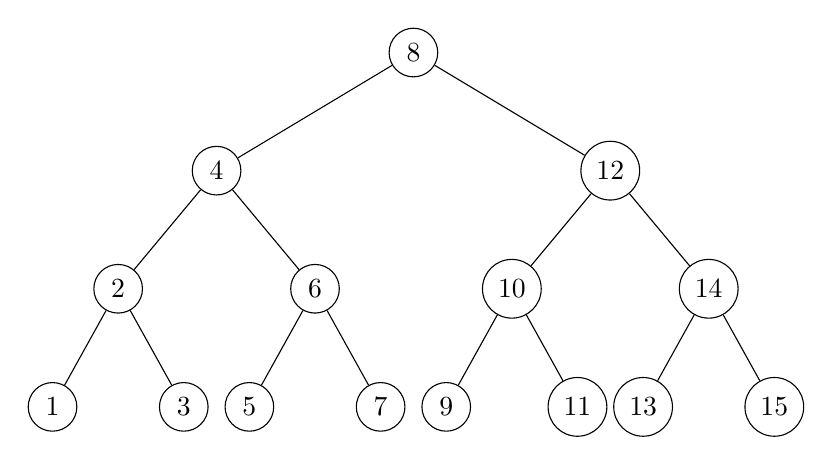
\begin{tikzpicture}[level/.style={sibling distance=50mm/#1}]
\node [circle,draw] (a){8}
  child {
  node [circle,draw] (b) {4}
    child {
    node [circle,draw] (c) {2}
        child {
            node [circle,draw] (d) {1}
        }
            child {
                node [circle,draw] (e) {3}
            }
      }
    child {
    node [circle,draw] (f) {6}
        child {
            node [circle,draw] (g) {5}
        }
            child {
                node [circle,draw] (h) {7}
            }
  }
  }
  child {
  node [circle,draw] (i) {12}
    child {
    node [circle,draw] (j) {10}
        child {
            node [circle,draw] (k) {9}
        }
            child {
                node [circle,draw] (l) {11}
            }
      }
    child {
    node [circle,draw] (m) {14}
        child {
            node [circle,draw] (n) {13}
        }
            child {
                node [circle,draw] (o) {15}
            }
  }
  };
\end{tikzpicture}

We shorten NIL to N so that it can be more easily displayed in the document. The following has black height 2.

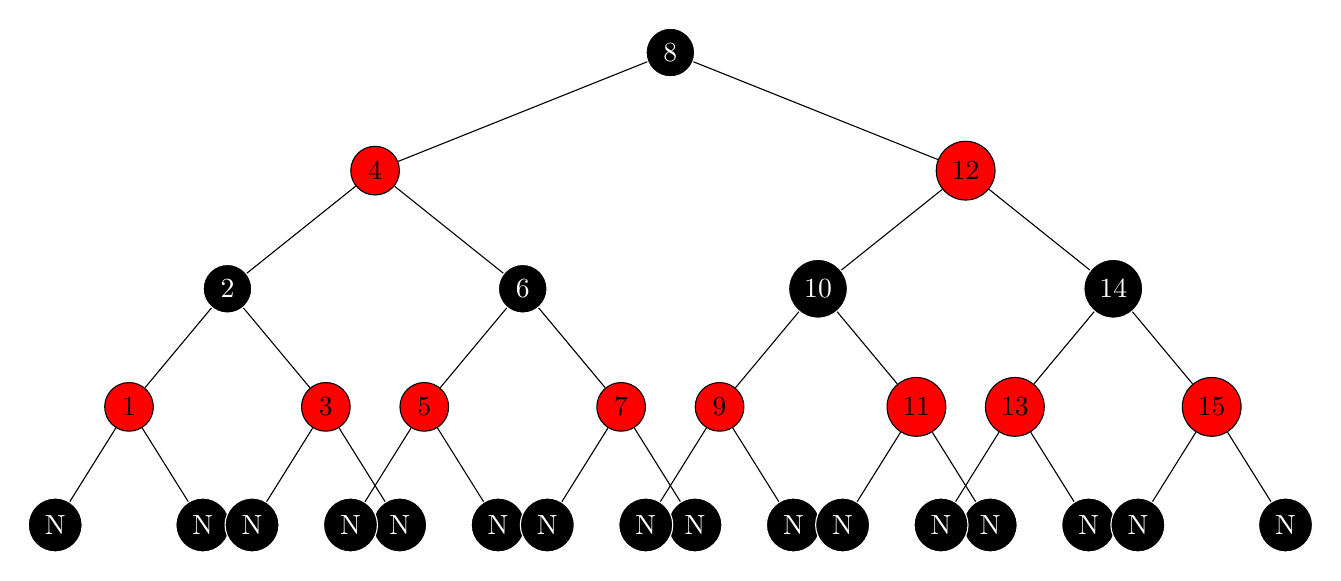
\begin{tikzpicture}[level/.style={sibling distance=75mm/#1}]
\node [circle,draw,color=white, fill=black] (a){8}
  child {
  node [circle,draw,fill =red] (b) {4}
    child {
    node [circle,draw,color=white, fill=black] (c) {2}
        child {
            node [circle,draw,fill =red] (d) {1}
            child{node [circle,draw,color=white, fill=black] (p) {N}}
            child{node [circle,draw,color=white, fill=black] (q) {N}}
        }
            child {
                node [circle,draw,fill =red] (e) {3}
            child{node [circle,draw,color=white, fill=black] (r) {N}}
            child{node [circle,draw,color=white, fill=black] (s) {N}}
            }
      }
    child {
    node [circle,draw,color=white, fill=black] (f) {6}
        child {
            node [circle,draw,fill =red] (g) {5}
            child{node [circle,draw,color=white, fill=black] (t) {N}}
            child{node [circle,draw,color=white, fill=black] (u) {N}}
        }
            child {
                node [circle,draw,fill =red] (h) {7}
            child{node [circle,draw,color=white, fill=black] (v) {N}}
            child{node [circle,draw,color=white, fill=black] (w) {N}}
            }
  }
  }
  child {
  node [circle,draw,fill =red] (i) {12}
    child {
    node [circle,draw,color=white, fill=black] (j) {10}
        child {
            node [circle,draw,fill =red] (k) {9}
            child{node [circle,draw,color=white, fill=black] (x) {N}}
            child{node [circle,draw,color=white, fill=black] (y) {N}}
        }
            child {
                node [circle,draw,fill =red] (l) {11}
            child{node [circle,draw,color=white, fill=black] (z) {N}}
            child{node [circle,draw,color=white, fill=black] (aa) {N}}
            }
      }
    child {
    node [circle,draw,color=white, fill=black] (m) {14}
        child {
            node [circle,draw,fill =red] (n) {13}
            child{node [circle,draw,color=white, fill=black] (ab) {N}}
            child{node [circle,draw,color=white, fill=black] (ac) {N}}
        }
            child {
                node [circle,draw,fill =red] (o) {15}
            child{node [circle,draw,color=white, fill=black] (ad) {N}}
            child{node [circle,draw,color=white, fill=black] (ae) {N}}
            }
  }
  };
\end{tikzpicture}

The following has black height 3

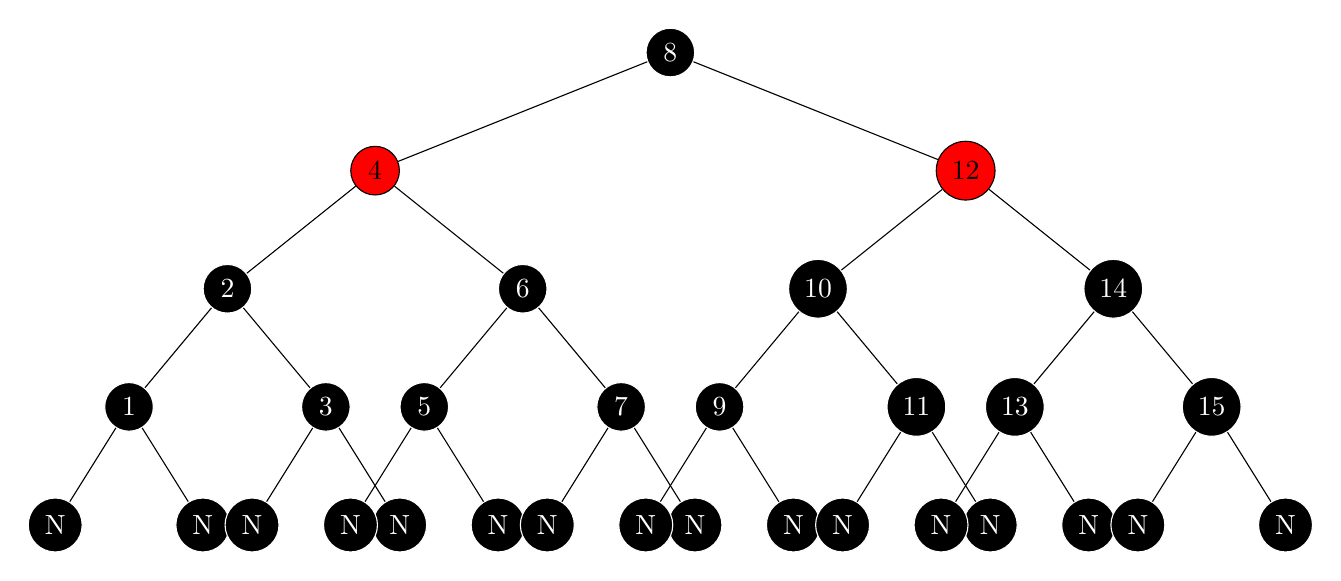
\begin{tikzpicture}[level/.style={sibling distance=75mm/#1}]
\node [circle,draw,color=white, fill=black] (a){8}
  child {
  node [circle,draw,fill =red] (b) {4}
    child {
    node [circle,draw,color=white, fill=black] (c) {2}
        child {
            node [circle,draw,color=white, fill=black] (d) {1}
            child{node [circle,draw,color=white, fill=black] (p) {N}}
            child{node [circle,draw,color=white, fill=black] (q) {N}}
        }
            child {
                node [circle,draw,color=white, fill=black] (e) {3}
            child{node [circle,draw,color=white, fill=black] (r) {N}}
            child{node [circle,draw,color=white, fill=black] (s) {N}}
            }
      }
    child {
    node [circle,draw,color=white, fill=black] (f) {6}
        child {
            node [circle,draw,color=white, fill=black] (g) {5}
            child{node [circle,draw,color=white, fill=black] (t) {N}}
            child{node [circle,draw,color=white, fill=black] (u) {N}}
        }
            child {
                node [circle,draw,color=white, fill=black] (h) {7}
            child{node [circle,draw,color=white, fill=black] (v) {N}}
            child{node [circle,draw,color=white, fill=black] (w) {N}}
            }
  }
  }
  child {
  node [circle,draw,fill =red] (i) {12}
    child {
    node [circle,draw,color=white, fill=black] (j) {10}
        child {
            node [circle,draw,color=white, fill=black] (k) {9}
            child{node [circle,draw,color=white, fill=black] (x) {N}}
            child{node [circle,draw,color=white, fill=black] (y) {N}}
        }
            child {
                node [circle,draw,color=white, fill=black] (l) {11}
            child{node [circle,draw,color=white, fill=black] (z) {N}}
            child{node [circle,draw,color=white, fill=black] (aa) {N}}
            }
      }
    child {
    node [circle,draw,color=white, fill=black] (m) {14}
        child {
            node [circle,draw,color=white, fill=black] (n) {13}
            child{node [circle,draw,color=white, fill=black] (ab) {N}}
            child{node [circle,draw,color=white, fill=black] (ac) {N}}
        }
            child {
                node [circle,draw,color=white, fill=black] (o) {15}
            child{node [circle,draw,color=white, fill=black] (ad) {N}}
            child{node [circle,draw,color=white, fill=black] (ae) {N}}
            }
  }
  };
\end{tikzpicture}

Lastly, the following has black height 4.

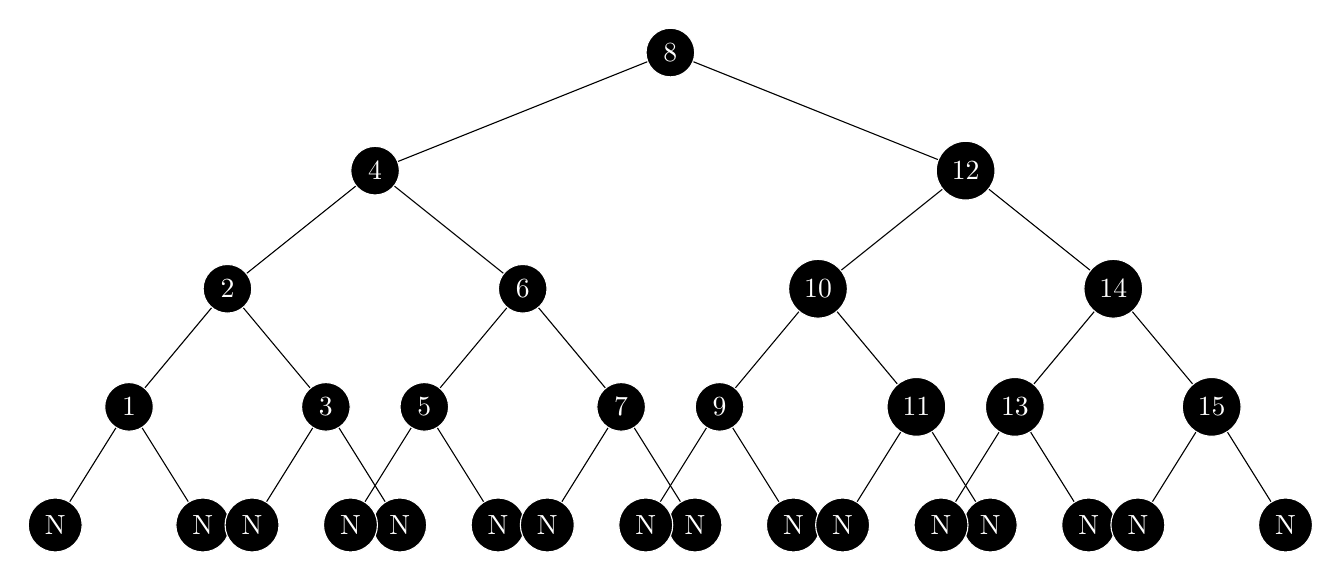
\begin{tikzpicture}[level/.style={sibling distance=75mm/#1}]
\node [circle,draw,color=white, fill=black] (a){8}
  child {
  node [circle,draw,color=white, fill=black] (b) {4}
    child {
    node [circle,draw,color=white, fill=black] (c) {2}
        child {
            node [circle,draw,color=white, fill=black] (d) {1}
            child{node [circle,draw,color=white, fill=black] (p) {N}}
            child{node [circle,draw,color=white, fill=black] (q) {N}}
        }
            child {
                node [circle,draw,color=white, fill=black] (e) {3}
            child{node [circle,draw,color=white, fill=black] (r) {N}}
            child{node [circle,draw,color=white, fill=black] (s) {N}}
            }
      }
    child {
    node [circle,draw,color=white, fill=black] (f) {6}
        child {
            node [circle,draw,color=white, fill=black] (g) {5}
            child{node [circle,draw,color=white, fill=black] (t) {N}}
            child{node [circle,draw,color=white, fill=black] (u) {N}}
        }
            child {
                node [circle,draw,color=white, fill=black] (h) {7}
            child{node [circle,draw,color=white, fill=black] (v) {N}}
            child{node [circle,draw,color=white, fill=black] (w) {N}}
            }
  }
  }
  child {
  node [circle,draw,color=white, fill=black] (i) {12}
    child {
    node [circle,draw,color=white, fill=black] (j) {10}
        child {
            node [circle,draw,color=white, fill=black] (k) {9}
            child{node [circle,draw,color=white, fill=black] (x) {N}}
            child{node [circle,draw,color=white, fill=black] (y) {N}}
        }
            child {
                node [circle,draw,color=white, fill=black] (l) {11}
            child{node [circle,draw,color=white, fill=black] (z) {N}}
            child{node [circle,draw,color=white, fill=black] (aa) {N}}
            }
      }
    child {
    node [circle,draw,color=white, fill=black] (m) {14}
        child {
            node [circle,draw,color=white, fill=black] (n) {13}
            child{node [circle,draw,color=white, fill=black] (ab) {N}}
            child{node [circle,draw,color=white, fill=black] (ac) {N}}
        }
            child {
                node [circle,draw,color=white, fill=black] (o) {15}
            child{node [circle,draw,color=white, fill=black] (ad) {N}}
            child{node [circle,draw,color=white, fill=black] (ae) {N}}
            }
  }
  };
\end{tikzpicture}\\

\noindent\textbf{ Exercise 13.1-3} \\
It will. There was no red node introduced, so 4 will still be satisfied. Since the root is in every path from the root to the leaves, but no others. 5 will be satisfied because the only paths we will be changing the number of black nodes in are those coming from the root. All of these will increase by 1, and so will all be equal. 3 is trivially preserved, as no new leaves are introduced. 1 is also trivially preserved as only one node is changed and it is not changed to some mysterious third color.\

\noindent\textbf{ Exercise 13.1-5} \\
Suppose we have the longest simple path $(a_1,a_2,\ldots a_s)$ and the shortest simple path $(b_1,b_2, \ldots, b_t)$. Then, by propery 5 we know they have equal numbers of black nodes. By property 4, we know that neither contains a repeated red node. This tells us that at most $\lfloor\frac{s-1}{2}\rfloor$ of the nodes in the longest path are red. This means that at least $\lceil \frac{s+1}{2} \rceil$ are black, so, $t\ge \lceil \frac{s+1}{2} \rceil$. So, if, by way of contradiction, we had that $s>t*2$, then $  t \ge \lceil \frac{s+1}{2} \rceil \ge \lceil\frac{2t+2}{2} \rceil = t+1$ a contradiction.\\


\noindent\textbf{ Exercise 13.1-7} \\
Since each red node needs to have two black children, our only hope at getting a large number of internal red nodes relative to our number of black internal nodes is to make it so that the parent of every leaf is a red node. So, we would have a ratio of $\frac{2}{3}$ if we have the tree with a black root which has red children, and all of it's grandchildren be leaves. We can't do better than this because as we make the tree bigger, the ratio approaches $\frac{1}{2}$.

The smallest ratio is acheived by having a complete tree that is balanced and black as a raven's feather. For example, see the last tree presented in the solution to 13.1-1. \\

\noindent\textbf{ Exercise 13.2-1} \\
See the algorithm for RIGHT-ROTATE.\\


\begin{algorithm}
\caption{RIGHT-ROTATE(T,x)}
\begin{algorithmic}
\State y = x.left
\State x.left = y.right
\If{$y.right \neq T.nil$}
\State t.right.p = x
\EndIf
\State y.p = x.p
\If{x.p == T.nil}
\State T.root = y
\ElsIf{x == x.p.left}
\State x.p.left = y
\Else
\State x.p.right = y
\EndIf
\State y.right =x
\State x.p =y
\end{algorithmic}
\end{algorithm}

\noindent\textbf{ Exercise 13.2-3} \\
the depth of $c$ decreases by one, the depth of $b$ stays the same, and the depth of $a$ increases by 1.\\


\noindent\textbf{ Exercise 13.2-5} \\
Consider the BST for $T_2$ to be

\begin{tikzpicture}[level/.style={sibling distance=75mm/#1}]
\node [circle,draw] (a){8}
  child {
  node [circle,draw] (b) {4}
    child {node [circle,draw] (c) {NIL}
    }
      child {node [circle,draw] (d) {NIL}
      }
  }
  child{ node [circle,draw] (e) {NIL}};
\end{tikzpicture}

And let $T_1$ be 

    \begin{tikzpicture}[level/.style={sibling distance=75mm/#1}]
\node [circle,draw] (a){8}
  child{ node [circle,draw] (e) {NIL}}
  child {
  node [circle,draw] (b) {4}
    child {node [circle,draw] (c) {NIL}
    }
      child {node [circle,draw] (d) {NIL}
      }
  };
\end{tikzpicture}

Then, there are no nodes for which its valid to call right rotate in $T_1$. Even though it is possible to right convert $T_2$ into $T_1$, the reverse is not possible.


For any BST T, define the quantity $f(T)$ to be the sum over all the nodes of the number of left pointers that are used in a simple path from the root to that node. Note that the contribution from each node is $O(n)$. Since there are only $n$ nodes, we have that $f(T)$ is $O(n^2)$. Also, when we call RIGHT-ROTATE(T,x), then the contribution from $x$ decreases by one, and the contribution from all other elements remain the same. Since $f(T)$ is a quantity that decreases by exactly one with every call of RIGHT-ROTATE, and begins $O(n^2)$, and never goes negative, we know that there can only be at most $O(n^2)$ calls of RIGHT-ROTATE on a BST.\\



\noindent\textbf{ Exercise 13.3-1} \\



\noindent\textbf{ Exercise 13.3-3} \\
\noindent\textbf{ Exercise 13.3-5} \\
\noindent\textbf{ Exercise 13.4-1} \\

\end{document} 